\documentclass{beamer}
\usepackage[russian]{babel}
\usetheme{metropolis}

\usepackage{amsthm}
\setbeamertemplate{theorems}[numbered]

\setbeamercolor{block title}{use=structure,fg=white,bg=gray!75!black}
\setbeamercolor{block body}{use=structure,fg=black,bg=gray!20!white}

\usepackage[T2A]{fontenc}
\usepackage[utf8]{inputenc}

\usepackage{hyphenat}
\usepackage{amsmath}
\usepackage{graphicx}

\AtBeginEnvironment{proof}{\renewcommand{\qedsymbol}{}}{}{}

\title{
Микроэкономика-I
}
\author{
Павел Андреянов, PhD
}

\begin{document}
\maketitle

\section{План}

\begin{frame}{План}
	
Мы продолжаем разбор теории производителя.

\textbf{Первая часть лекции} посвящена средним и фиксированным издержкам, а также связанными с последним идеями о точках закрытия рынка и монополистической конкуренции.

\textbf{Вторая часть лекции} агрегированию и сдвигам кривых спроса и предложения, а также понятию частичного равновесия.
	
\end{frame}

\section{Средние издержки}

\begin{frame}{Средние издержки}
В этой секции я буду использовать $Q$ для обозначения объемов производства (не путать с ценами факторов $q$).

Несмотря на доминирование маржиналистского подхода в экономике, некоторые фирмы устанавливают объем производства так, чтобы средние издержки плюс какая-то субъективная (например, 10\%) маржа были равны рыночной цене. 

Это не имеет никакого смысла с точки зрения максимизации прибыли, так как прибыль в таком случае будет всегда равна нулю. Единственный смысл в том, что средние издержки легко считаются.

\end{frame}

\begin{frame}{Средние издержки}

\begin{definition}
\textbf{Средние издержки}, или ATC(Q), – это отношения общих издержек (TC(Q)) к объему производства:
$$ATC(Q) = TC(Q)/Q$$

\end{definition}

\end{frame}

\begin{frame}{Средние издержки}
Действительно, монопольная фирма использует правило обратной эластичности $-1 + P/MC(Q) = -1/\varepsilon$, а конкурентная фирма использует правило $P = MC(Q)$. 

Но у функции $ATC(Q)$ есть одно интересное свойство:

\begin{lemma}
Цена, при которой у конкурентной фирмы прибыль равна нулю, определяется любым из двух способов:
- это минимум ATC(Q) по Q
- это пересечение ATC(Q) и MC(Q)
\end{lemma}
В частности, это означает, что кривые ATC(Q) и MC(Q) пересекаются в той же точке, где у ATC(Q) минимум. Запомните эту картинку "трезубец":
\end{frame}

\begin{frame}{Средние издержки}
\begin{figure}[hbt]
\centering
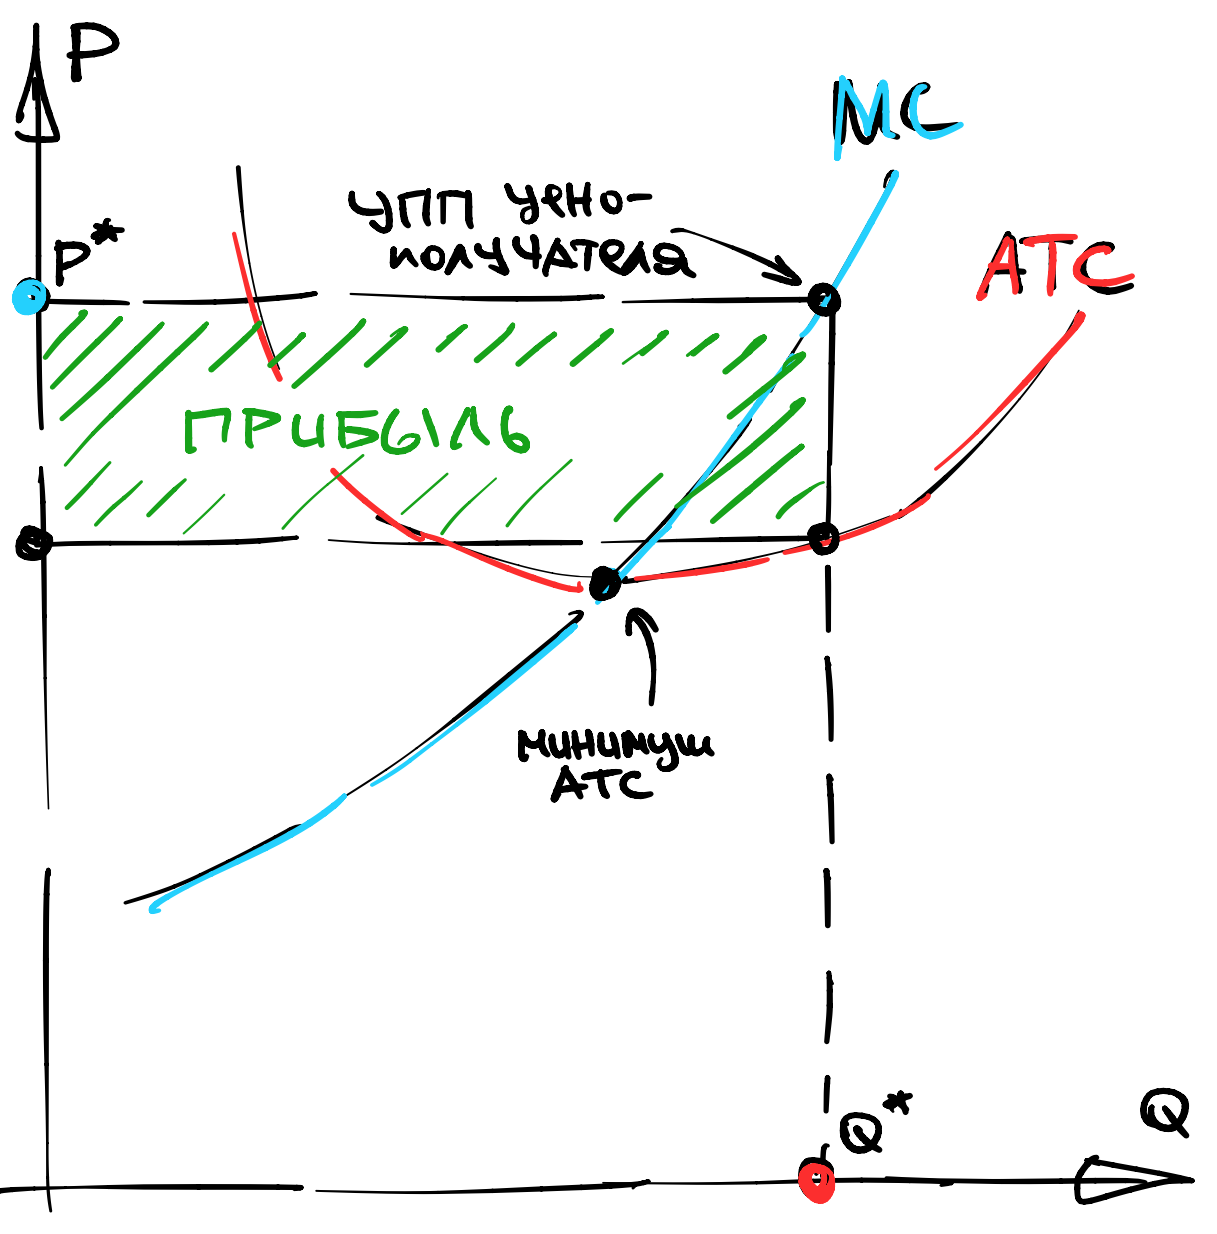
\includegraphics[width=.7 \textwidth]{trident.png}
\end{figure}
\end{frame}

\begin{frame}{Средние издержки}

Откуда берется такая форма? Из-за фиксированных издержек. Назовем переменными издержками $VC(Q) = TC(Q) - FC$, тогда
$$ ATC(Q) = \frac{FC}{Q} + \frac{VC(Q)}{Q}.$$

Заметим, что первый член убывает гиперболически, а второй член возрастает (как-то), потому что функция $TC(Q)$ выпукла, а значит выпукла $VC(Q)$, а значит должна расти сверхлинейно, ну или хотя бы линейно.

Поэтому, считается что $ATC(Q)$ имеет U-образную форму. 

Единственный случай, когда это неверно - это когда фиксированных издержек нет совсем.

\end{frame}

\section{Точка закрытия в долгосрочном периоде}

\begin{frame}{ТЗ в долгосрочном периоде}

На той же картинке <<трезубец>> мы можем изобразить прибыль фирмы - это площадь прямоугольника со сторонами $Q$ и $ATC(Q)-P$. 

\begin{definition}
Назовем пересечение $MC(Q)$ с $ATC(Q)$ \textbf{точкой закрытия в долгосрочном периоде}, я буду использовать обозначение $MC \cap ATC$.
\end{definition}

Почему в долгосрочном? Потому, что фиксированные издержки (завод, лицензия...) можно <<отбить>> только в долгосрочном периоде. 

\end{frame}

\begin{frame}{ТЗ в долгосрочном периоде}

Очевидно следующее

\begin{lemma}
Если цена падает ниже уровня $MC \cap ATC$, то производитель готов уйти с рынка в долгосрочном периоде.
\end{lemma}

Что означает закрытие в долгосрочном периоде на практике? Например, хозяин бизнеса увольняет всех рабочих, распродает активы и уходит (с деньгами) с рынка.

А что будет происходить в краткосрочном периоде?

\end{frame}

\section{Точка закрытия в краткосрочном периоде}

\begin{frame}{ТЗ в краткосрочном периоде}

Поразительно, но если цена падает ниже уровня $MC \cap ATC$ в краткосрочном периоде, то производитель какое-то время может продолжать работать в убыток.

Почему?

Дело в том, что в краткосрочном периоде производитель не воспринимает константу FC как что-то в его власти. Поэтому везде он видит переменные издержки вместо общих.
\end{frame}

\begin{frame}{ТЗ в краткосрочном периоде}

\begin{definition}
\textbf{Средние переменные издержки}, или AVC(Q), – это отношение переменных издержек VC(Q)) к объему производства:
$$AVC(Q) = VC(Q)/Q = (TC(Q) - FC)/Q$$
\end{definition}

На той же картинке <<трезубец>> мы можем изобразить прибыль фирмы за вычетом фиксированных издержек - это площадь прямоугольника со сторонами $Q$ и $AVC(Q)-P$. 

\end{frame}

\begin{frame}{ТЗ в краткосрочном периоде}

\begin{figure}[hbt]
\centering
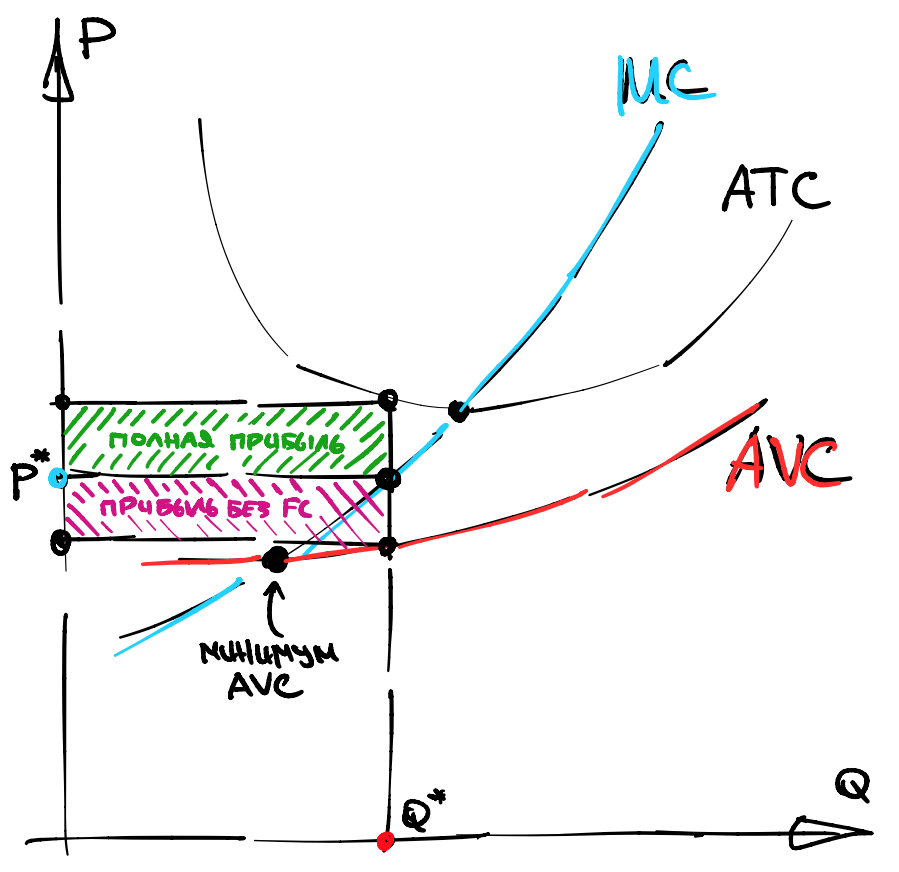
\includegraphics[width=.7 \textwidth]{trident2.png}
\end{figure}

\end{frame}


\begin{frame}{ТЗ в краткосрочном периоде}

\begin{definition}
Назовем пересечение $MC$ с $AVC$ \textbf{точкой закрытия в краткосрочном периоде}, я буду использовать обозначение $MC \cap AVC$.
\end{definition}

Эта новая точка закрытия не выше предыдущей, поскольку AVC всегда не выше ATC. Если цена продолжает падать и достигает этого, более низкого, уровня, то прибыль, даже без учета FC, становится нулевой.

\end{frame}

\begin{frame}{ТЗ в краткосрочном периоде}

\begin{lemma}
Если цена падает ниже уровня $MC \cap AVC$, то производитель останавливает производство в краткосрочном периоде.
\end{lemma}

Что означает закрытие в краткосрочном периоде на практике?

\end{frame}

\begin{frame}{ТЗ в краткосрочном периоде}

Это означает, что завод стоит, но на нем никто ничего не производит, то есть $Q=0$. 

Сторож охраняет вход, а владелец бизнеса ждет, когда цена отскочит назад, и постепенно думает, кому бы продать завод в краткосрочном периоде.

\end{frame}

\section{Пример}

\begin{frame}{Пример}

Рассмотрим два завода: высокотехнологичный и "так себе". 

Высокотехнологичный завод обладает высокими фиксированными издержками, но низкими переменными:
$$FC_1 = 2, \quad VC_1(Q) = Q + Q^2/2, \quad MC_1(Q) = 1 + Q$$

"Так себе" завод организован в поле, поэтому обладает нулевыми фиксированными издержками, но высокими переменными:
$$FC_2 = 0, \quad VC_2(Q) = 2Q + Q^2, \quad MC_2(Q) = 2 + 2Q.$$

\end{frame}

\begin{frame}{Пример}

Рассмотрим два завода: высокотехнологичный и "так себе". 

Высокотехнологичный завод обладает высокими фиксированными издержками, но низкими переменными:
$$FC_1 = 2, \quad VC_1(Q) = Q + Q^2/2, \quad MC_1(Q) = 1 + Q$$

"Так себе" завод организован в поле, поэтому обладает нулевыми фиксированными издержками, но высокими переменными:
$$FC_2 = 0, \quad VC_2(Q) = 2Q + Q^2, \quad MC_2(Q) = 2 + 2Q$$

Проанализируем точки закрытия каждого из этих заводов в долгосрочном периоде.

\end{frame}

\begin{frame}{Пример}
	
Для первого завода это решение уравнения:

\begin{gather*}
(1+Q) Q = 2 + Q + Q^2/2 \\
Q^2/2 = 2\\
Q = 2
\end{gather*}

Нам повезло – корень целый, и в точке закрытия высокотехнологичного завода цена равна $P=3$. 
	
\end{frame}

\begin{frame}{Пример}

Для второго завода это решение уравнения:

\begin{gather*}
(2+2Q) Q = 2Q + Q^2 \\
2Q = Q\\
Q = 0
\end{gather*}

В точке закрытия "так себе" завода цена равна $P=2$.
	
\end{frame}

\begin{frame}{Пример}

Какой из этого можно сделать вывод?
	
\end{frame}

\begin{frame}{Пример}

При падении цены первыми терпеть убытки начинают высокотехнологичные заводы. Низкотехнологичные заводы продолжают какое-то время получать прибыль из-за того, что их фиксированные издержки малы.
	
\end{frame}

\section{Монополистическая конкуренция}

\begin{frame}{Монополистическая конкуренция}

Предположим, что есть убывающая кривая спроса на товар, скажем, $P(Q) = 100 - Q$ и фирмы могут свободно заходить и выходить с рынка.

Предположим также, что у каждой фирмы есть фиксированные издержки входа на рынок, равные FC. Понятно, что весь излишек потребителя конечен - это площадь под кривой. С другой стороны, каждая фирма платит FC за вход, значит, количество фирм не может быть очень большим.
	
\end{frame}

\begin{frame}{Монополистическая конкуренция}

\begin{definition}
Назовем \textbf{долгосрочным равновесием, или равновесием в монополистической конкуренции}, максимальное число фирм, такое, что их прибыль (в долгосрочном периоде) неотрицательна, а также равновесную цену и соответствующие объемы производства.
\end{definition}

\end{frame}

\section{Пример}

\begin{frame}{Пример}

Рассмотрим пример поиска такого равновесия.

\begin{itemize}
\item пусть есть много идентичных фирм
\item обозначим суммарный спрос за $Q_{\sum} = \sum Q_i$
\item пусть спрос описывается $P(Q_{\sum}) = 100 - Q_{\sum}$
\item пусть издержки описываются $FC = 1, \ VC(Q_i) = Q_i^2/2$
\end{itemize}

\end{frame}

\begin{frame}{Пример}

Пусть $n$ – это число фирм. Каждая фирма выбирает $Q_i$ так, что $P = MC(Q_i)$, то есть в нашем случае, $Q_i = P$. Это значит, что суммарное предложение равно: 

$$Q_{\sum} = n Q_i = n P.$$

\end{frame}

\begin{frame}{Пример}

Теперь найдем $n$, такое, что цена опустится в точку закрытия. Для этого запишем $MC, ATC$:
$$ MC(Q_i) = Q_i, \quad ATC(Q_i) = Q_i/2 + 1/Q$$

Приравнив их друг к другу, мы получим:
$$ MC(Q_i) = ATC(Q_i) \quad \Rightarrow \quad Q_i = \sqrt{2}$$

\end{frame}

\begin{frame}{Пример}

Теперь надо соединить вместе оптимальное поведение фирмы, условие на закрытие рынка и формулу спроса:
\begin{gather*}
P = 100 - n Q_i,\\
Q_i = P,\\
Q_i = \sqrt{2}.
\end{gather*}

\end{frame}

\begin{frame}{Пример}

Это система из трех уравнений и трех неизвестных, откуда мы можем вычислить число фирм, которое обеспечит неотрицательную прибыль, но только надо взять ближайшее целое число снизу:
$$100/\sqrt{2} - 1 \approx 69,$$

С 69 фирмами прибыль будет слишком маленькой для того, чтобы новая фирма вошла на рынок, но все же положительной.

\end{frame}

\begin{frame}{Пример}
Чтобы найти ее, надо пересчитать все заново.
\begin{gather*}
P = 100 - 69 Q_i\\
Q_i = P
\end{gather*}
Получится $P = Q_i = 10/7$. Выручка равна приблизительно $2.04$, фиксированные издержки равны $1$ переменные издержки примерно $1.02$. 

Соответственно, прибыль фирмы равна примерно $0.02$.

\end{frame}

\section{Перерыв}

\end{document}